% ACS Environmental Science & Technology Manuscript Template
% Using achemso document class

\documentclass[
  journal=esthag,        % Environmental Science & Technology
  manuscript=article,    % Research Article
  layout=twocolumn       % Two-column layout for review
]{achemso}

% Required packages
\usepackage[version=4]{mhchem}    % Chemical formulas
\usepackage{siunitx}              % SI units
\usepackage{graphicx}             % Figures
\usepackage{booktabs}             % Professional tables
\usepackage{multirow}             % Table formatting
\usepackage{xcolor}               % Colors

% Graphics path
\graphicspath{{Data/}}

% ============================================================================
% AUTHOR INFORMATION
% ============================================================================

\author{Isaac A. Author}
\affiliation{Department of Earth System Science, University of California, Irvine, CA 92697, United States}
\email{author@uci.edu}

\author{Second Author}
\affiliation{NASA Jet Propulsion Laboratory, California Institute of Technology, Pasadena, CA 91109, United States}

% ============================================================================
% TITLE
% ============================================================================

\title{Metal Contamination in Wildfire Ash from the 2025 Eaton Fire: Field-Portable XRF Calibration for Rapid Screening}

% ============================================================================
% ABSTRACT (150-200 words)
% ============================================================================

\begin{abstract}
Wildfire ash from urban-wildland interface fires contains elevated concentrations of toxic metals that pose risks to human health and ecosystems during post-fire recovery. We characterized metal concentrations in 39 ash samples collected from the 2025 Eaton Fire burn perimeter using ICP-MS and evaluated field-portable XRF as a rapid screening tool. Lead (Pb) concentrations ranged from 14 to 18,528 ppm (mean 638 ppm), with zinc (100--23,829 ppm) and copper (14--3,650 ppm) similarly elevated. Spatial heterogeneity was pronounced, with coefficients of variation exceeding 280\% for Pb, Zn, and Cu. We developed empirical calibrations for XRF using cumulative Pb L-line intensities, achieving $R^2$ = 0.994 and RMSE = 230 ppm against ICP-MS. Classification performance for regulatory screening thresholds reached 100\% sensitivity at 1000 ppm and 86\% sensitivity at 200 ppm, with no false positives. These results demonstrate that field-portable XRF with site-specific calibration enables rapid identification of highly contaminated areas during emergency response, supporting prioritization of remediation efforts.
\end{abstract}

% ============================================================================
% SYNOPSIS STATEMENT (Required by ES&T, ~20 words, after abstract)
% ============================================================================

% Synopsis: This study develops field-portable XRF methods for rapid screening
% of metal contamination in wildfire ash, enabling faster emergency response
% and targeted remediation.

% ============================================================================
% KEYWORDS (5-8 keywords)
% ============================================================================

\keywords{wildfire ash, urban-wildland interface, metal contamination, XRF calibration, lead, emergency response, screening levels}

% ============================================================================
% DOCUMENT BEGINS
% ============================================================================

\begin{document}

% ============================================================================
% INTRODUCTION
% ============================================================================

\section{Introduction}

% Introduction should establish context, identify knowledge gaps, and state objectives
% Typically 3-5 paragraphs, ~500-800 words

Wildfire activity in the western United States has intensified in recent decades, with increasing encroachment into urban-wildland interface (WUI) zones where residential structures intermix with combustible vegetation. The combustion of anthropogenic materials in WUI fires releases a complex mixture of contaminants distinct from wildland fires, including heavy metals from building materials, electronics, batteries, vehicles, and household products.

Lead contamination is of particular concern given its neurotoxic effects, especially for children, and the absence of a safe exposure threshold. Zinc, copper, and other metals released during structure combustion can further contribute to ecological toxicity in receiving waters during post-fire runoff. Rapid characterization of metal contamination is essential for emergency response, but laboratory analysis by inductively coupled plasma mass spectrometry (ICP-MS) requires days to weeks, delaying remediation decisions.

Field-portable X-ray fluorescence (XRF) spectrometry offers a potential solution for rapid on-site screening. However, matrix effects in heterogeneous ash samples and potential spectral interferences (e.g., As K$\alpha$ overlap with Pb L$\alpha$) may compromise quantitative accuracy. Site-specific calibration against laboratory standards is therefore necessary to establish reliable screening thresholds.

The objectives of this study were to: (1) characterize metal concentrations and spatial variability in ash from the 2025 Eaton Fire, (2) develop and validate empirical XRF calibration models against ICP-MS, and (3) evaluate classification performance for regulatory screening thresholds relevant to residential exposure scenarios.

% ============================================================================
% MATERIALS AND METHODS
% ============================================================================

\section{Materials and Methods}

\subsection{Study Area and Sample Collection}

The Eaton Fire ignited on January 7, 2025, in Altadena and Pasadena, California, burning approximately 14,000 acres and destroying over 7,000 structures. Ash samples (n = 39) were collected from residential properties within the burn perimeter between January 15--25, 2025. Sample locations were recorded using handheld GPS (Garmin GPSMAP 67i; $\pm$3 m accuracy). At each site, composite samples were collected from the top 5 cm of ash deposits, homogenized in the field, and stored in polyethylene bags for transport.

\subsection{ICP-MS Analysis}

Samples were digested using EPA Method 3051A (microwave-assisted acid digestion with HNO$_3$/HCl) and analyzed by ICP-MS (Agilent 7900) for 54 elements following EPA Method 6020B. Quality control included method blanks, laboratory control samples, and certified reference materials (NIST SRM 2710a Montana Soil). Recoveries for target analytes ranged from 85--115\%.

\subsection{XRF Analysis}

Field-portable XRF measurements were performed using a Thermo Scientific Niton XL3t GOLDD+ analyzer in Mining Cu/Zn mode (60 s measurement time). Each sample was analyzed in triplicate on pressed pellets. The instrument reports concentrations derived from fundamental parameters (FP) algorithms based on Pb L$\alpha$ emission, as well as raw emission line intensities (counts/s) for individual L-lines.

\subsection{Calibration Approach}

Two calibration models were compared:
\begin{enumerate}
  \item \textbf{FP model}: ICP-MS Pb (ppm) regressed against XRF-reported mass fraction (\%)
  \item \textbf{L-line model}: ICP-MS Pb (ppm) regressed against cumulative L-line intensity (L$\alpha$ + L$\beta$ counts/s)
\end{enumerate}

Model performance was evaluated by $R^2$, root mean square error (RMSE), and Akaike Information Criterion (AIC). Classification performance was assessed at regulatory screening thresholds of 80, 200, 400, and 1000 ppm Pb.

% ============================================================================
% RESULTS AND DISCUSSION
% ============================================================================

\section{Results and Discussion}

\subsection{Metal Concentrations in Wildfire Ash}

ICP-MS analysis quantified 54 elements in 39 ash samples collected within the Eaton Fire burn perimeter. Calcium dominated ash composition (mean 52,728 ppm; range 10,148--322,441 ppm), followed by aluminum (36,613 ppm), iron (36,577 ppm), potassium (18,858 ppm), magnesium (13,947 ppm), and sodium (13,271 ppm) (Table~\ref{tab:major_elements}).

Lead, zinc, and copper were the dominant trace contaminants. Zinc concentrations ranged from 100 to 23,829 ppm (mean 1,310 ppm), while lead ranged from 14 to 18,528 ppm (mean 638 ppm). Copper concentrations spanned 14--3,650 ppm (mean 207 ppm). These metals exhibited pronounced spatial heterogeneity, with coefficients of variation exceeding 280\% (Table~\ref{tab:trace_metals}).

% Insert Table 1 here
\begin{table}[htbp]
\caption{Major element concentrations (ppm) in Eaton Fire ash (n = 39).}
\label{tab:major_elements}
\begin{tabular}{lrrrr}
\toprule
Element & Mean & Median & Range & CV (\%) \\
\midrule
Ca & 52,728 & 33,378 & 10,148--322,441 & 116 \\
Fe & 36,577 & 38,332 & 8,336--64,081 & 37 \\
Al & 36,613 & 43,973 & 1,912--56,585 & 45 \\
K & 18,858 & 19,522 & 3,101--35,972 & 31 \\
Mg & 13,947 & 11,876 & 1,089--117,363 & 125 \\
Na & 13,271 & 14,451 & 3,731--22,361 & 37 \\
Ti & 6,138 & 5,246 & 3,171--19,222 & 55 \\
Mn & 962 & 898 & 273--2,742 & 48 \\
\bottomrule
\end{tabular}
\end{table}

% Insert Table 2 here
\begin{table}[htbp]
\caption{Trace metal concentrations (ppm) in Eaton Fire ash (n = 39), ordered by coefficient of variation.}
\label{tab:trace_metals}
\begin{tabular}{lrrrr}
\toprule
Element & Mean & Median & Range & CV (\%) \\
\midrule
Pb & 638 & 61 & 14--18,528 & 464 \\
Zn & 1,310 & 333 & 100--23,829 & 292 \\
Cu & 207 & 61 & 14--3,650 & 284 \\
Co & 22 & 14 & 5--216 & 150 \\
Ni & 46 & 26 & 17--372 & 143 \\
Sb & 9.1 & 4.1 & 2--49 & 135 \\
Cr & 55 & 43 & 22--332 & 91 \\
Cd & 0.5 & 0.3 & 0.1--1.5 & 74 \\
As & 6.5 & 6.1 & 3--12 & 33 \\
V & 85 & 82 & 20--143 & 31 \\
\bottomrule
\end{tabular}
\end{table}

\subsection{XRF Calibration Performance}

Linear regression models calibrating XRF against ICP-MS Pb concentrations demonstrated strong agreement (Table~\ref{tab:xrf_calibration}, Figure~\ref{fig:xrf_calibration}). The cumulative L-line model ($R^2$ = 0.994, RMSE = 230 ppm) outperformed the FP model ($R^2$ = 0.980, RMSE = 431 ppm), with substantial support from model comparison ($\Delta$AIC = 44).

% Insert Table 3 here
\begin{table}[htbp]
\caption{Linear regression models for XRF calibration of Pb against ICP-MS (n = 35).}
\label{tab:xrf_calibration}
\begin{tabular}{lrrrr}
\toprule
Model & $R^2$ & RMSE (ppm) & Slope (SE) & $\Delta$AIC \\
\midrule
Cumulative L-lines & 0.994 & 230 & 0.817 (0.011) & 0 \\
FP m.f.\% & 0.980 & 431 & 5,732 (141) & 44.2 \\
\bottomrule
\end{tabular}
\end{table}

% Insert Figure 1 here
\begin{figure}[htbp]
\centering
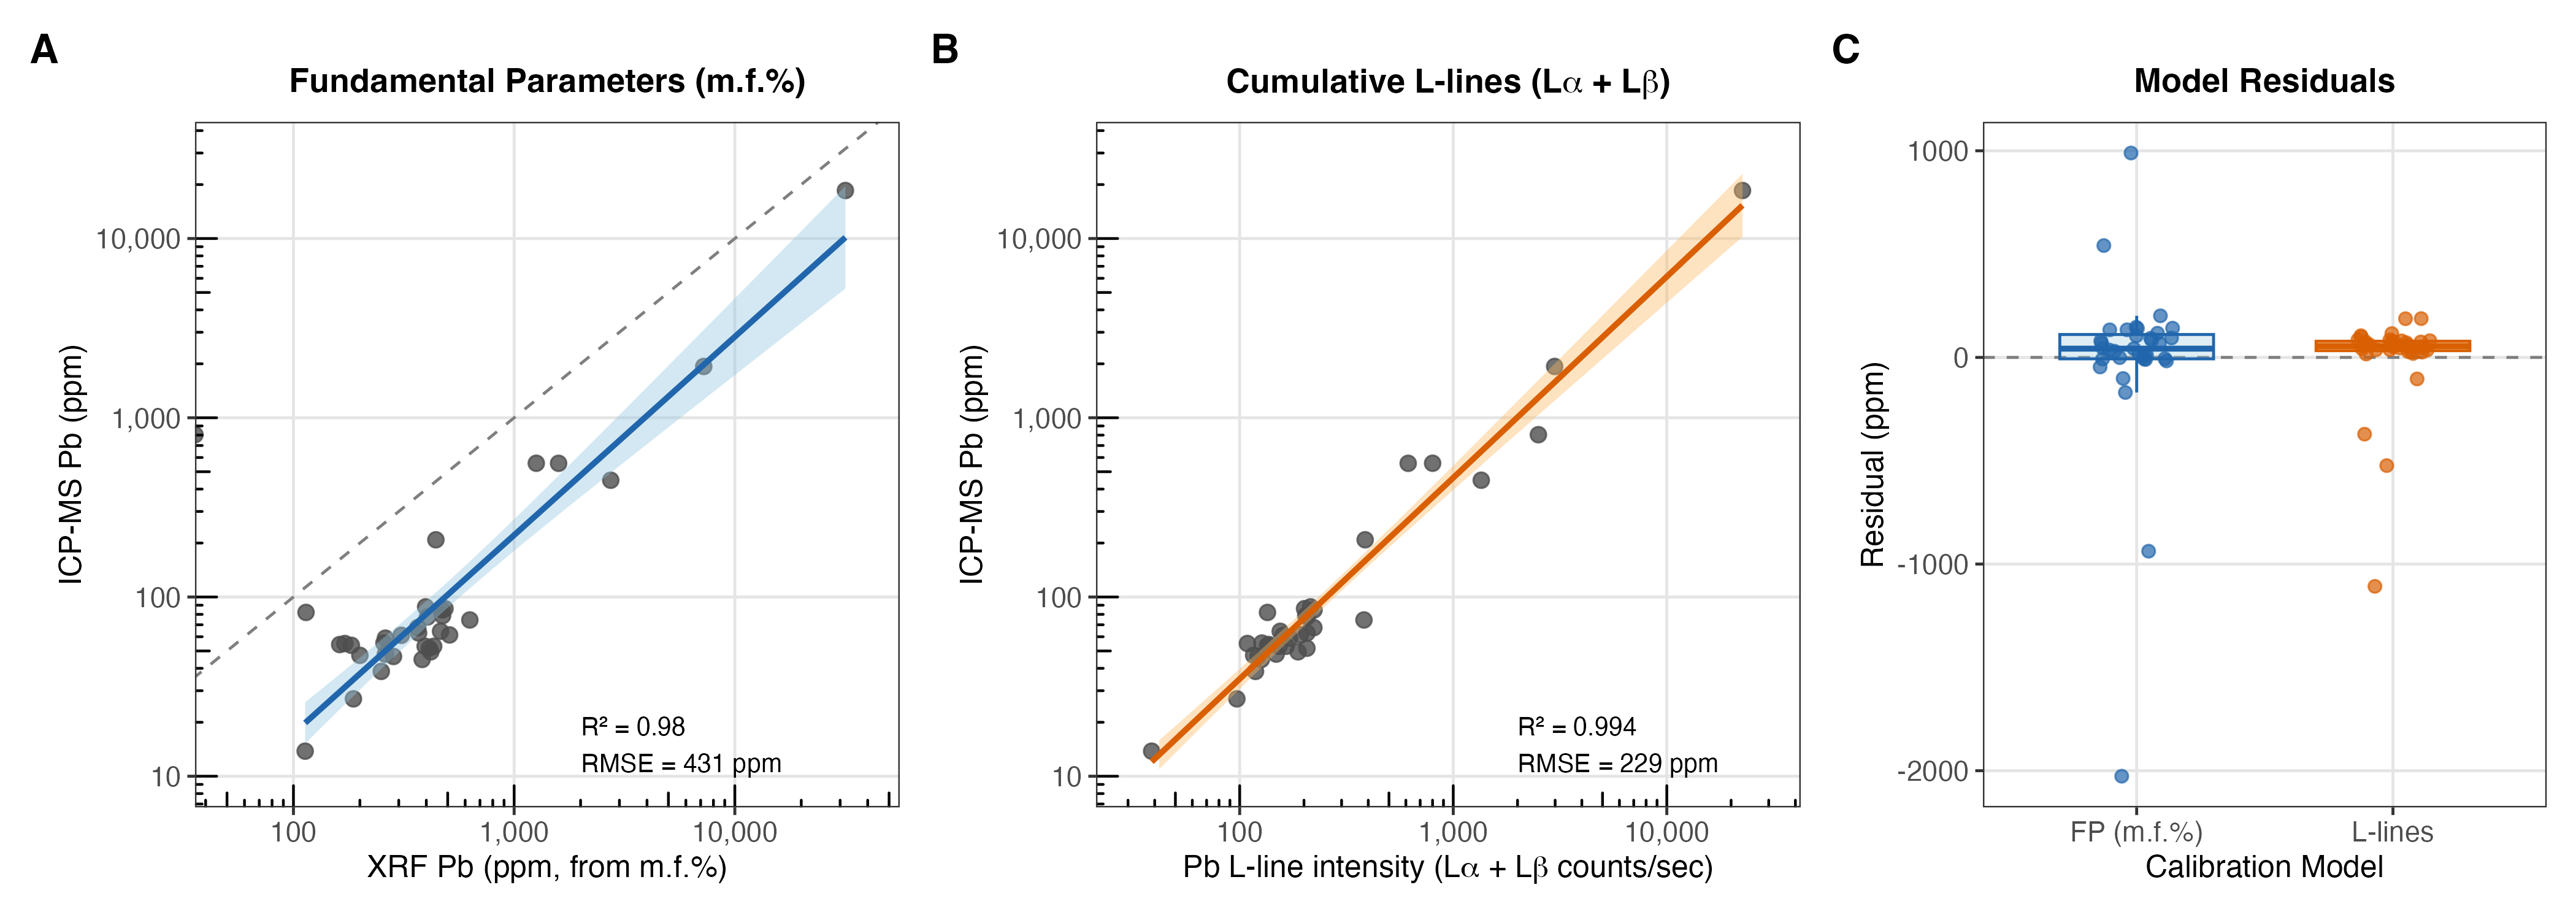
\includegraphics[width=\columnwidth]{Fig_XRF_calibration_final.png}
\caption{XRF calibration models for Pb quantification against ICP-MS (n = 35). Log-log scale. (A) Fundamental parameters model using manufacturer-reported m.f.\%. (B) Cumulative L-line intensity model (L$\alpha$ + L$\beta$). (C) Residual distributions for each calibration approach.}
\label{fig:xrf_calibration}
\end{figure}

\subsection{Screening Threshold Classification}

Classification performance improved with increasing threshold concentration (Table~\ref{tab:threshold_classification}). The cumulative L-line model achieved 100\% sensitivity at 1000 ppm, 83\% at 400 ppm, and 86\% at 200 ppm, with 100\% specificity (no false positives) at thresholds $\geq$200 ppm. At the 80 ppm threshold, sensitivity declined to 64\%, reflecting increased uncertainty at concentrations approaching the calibration intercept.

% Insert Table 4 here
\begin{table}[htbp]
\caption{Classification performance of calibrated XRF models for Pb screening thresholds (n = 35).}
\label{tab:threshold_classification}
\begin{tabular}{llrrrr}
\toprule
Threshold & Model & Sens. & Spec. & FP & FN \\
\midrule
80 ppm & L-lines & 64\% & 96\% & 1 & 4 \\
 & FP (m.f.\%) & 64\% & 83\% & 4 & 4 \\
200 ppm & L-lines & 86\% & 100\% & 0 & 1 \\
 & FP (m.f.\%) & 71\% & 100\% & 0 & 2 \\
400 ppm & L-lines & 83\% & 100\% & 0 & 1 \\
 & FP (m.f.\%) & 83\% & 100\% & 0 & 1 \\
1000 ppm & L-lines & 100\% & 97\% & 1 & 0 \\
 & FP (m.f.\%) & 100\% & 97\% & 1 & 0 \\
\bottomrule
\end{tabular}
\end{table}

\subsection{Implications for Emergency Response}

These results demonstrate that field-portable XRF with site-specific calibration can reliably identify samples exceeding moderate-to-high regulatory thresholds ($\geq$200 ppm) but may underestimate contamination at lower screening levels. The absence of false positives at thresholds $\geq$200 ppm is particularly important for emergency response, as it prevents unnecessary evacuation or remediation of uncontaminated areas while ensuring that highly contaminated sites are identified for priority action.

% ============================================================================
% ASSOCIATED CONTENT
% ============================================================================

\begin{suppinfo}

Supporting Information is available free of charge on the ACS Publications website.

\begin{itemize}
  \item Additional figures showing spatial distribution of metal concentrations (PDF)
  \item Complete ICP-MS dataset for all 54 elements (XLSX)
  \item XRF emission line intensity data (CSV)
\end{itemize}

\end{suppinfo}

% ============================================================================
% AUTHOR INFORMATION
% ============================================================================

\begin{acknowledgement}
This work was supported by [funding source]. We thank [acknowledgments].
\end{acknowledgement}

% ============================================================================
% REFERENCES
% ============================================================================

\bibliography{references}

\end{document}
